\documentclass[a4paper,10pt]{article}
\usepackage[margin=1in]{geometry}
\usepackage{polski}
\usepackage[utf8x]{inputenc}
\usepackage[unicode]{hyperref}
\usepackage{amssymb}
\usepackage{xifthen}
\usepackage[fleqn]{amsmath}
\usepackage{todonotes}
\usepackage{graphicx}
\usepackage{float}
\usepackage{fullpage}
\usepackage{epstopdf}
\usepackage{multirow}
\usepackage{subfig}
\usepackage[europeanresistors,americaninductors]{circuitikz}
\usetikzlibrary{patterns}
\newcommand{\withtodo}{0}


\def\arraystretch{1.2}


\begin{document}

\begin{table}
  \centering
  \def\arraystretch{1.5}
    \begin{tabular}{|l|l|l|l|} \hline
    Wydział:           & \multicolumn{2}{l|}{Dzień:Poniedziałek 14-17}    &Zespół:  \\
    Fizyki             &    \multicolumn{2}{l|}{Data: 20.03.2017}         &8             \\\hline
    Imiona i nazwiska: &Ocena z przygotowania:  &Ocena ze sprawozdania:   &Ocena końcowa: \\
    Marta Pogorzelska  &                        &                         &                \\
    Paulina Marikin    &                        &                         &\\\hline
    \multicolumn{2}{|l|}{Prowadzący:                 } &\multicolumn{2}{l|}{Podpis:             }  \\\hline
  \end{tabular}
\end{table}

\title{Ćwiczenie 30:\\Odbicie światła od powierzchni dielektryka}
\date{}
\maketitle

\section{Cel badań}
Celem doświadczenia było zweryfikowanie poprawności prawa Snella i prawa Malusa oraz wyznaczenie
kąta granicznego, kąta Brusnela i wspówłczynnika załamania badanego dielektryka.

\section{Wstęp teoretyczny}
\subsection{Prawo Snella}
Fala elektromagnetyczna na granicy ośrodków ulega dwóm zjawiską: załamaniu i odbiciu, gdzie fala załamana jest częścią fali, która zmieniła
ośrodek, zaś fala odbita częścią pozostałą w pierwotnym ośrodku. Kąty pod jakimi rozchodza się te fale (mierzone do normalnej - osi prostopadłej do płaszczyzny odbicia)
 są ze sobą powiązane przez prawo Snella:
\begin{equation}
    n_1\sin{\alpha} = n_2\sin{\beta}
\end{equation}
Kąt $\aplha$ jest kątem odbicia równym kątowi padania, $\beta$ to kąt załamania, zaś $n_1$ i $n_2$ to współczynniki załamania definiowane $n = \frac{c}{v}$
,gdzie v - prędkość fali elektromagnetycznej w danym ośrodku. Po przekształceniu
\begin{equation}
n_2 = n_1 \frac{\sin{\alpha}}{\sin{\beta}}
\end{equation}
można na podstawie prawa Snella wyznaczyć eksperymentalnie współczynnik załamania danego ośrodka.
\subsection{Kąt Brewstera}
Na potrzeby badanego zjawiska fale spolaryzowaną rozważymy jako nałożenie się dwóch fal o prostopadłych polaryzacjach, z wektorem
pola elektrycznego prostopadłym($\sigma$) i równoległym($\pi$) do płaszczyzny padania. Fala odbita złożona jest z ułamków obu tych fal zależnych
od kąta padania, przy czym składowa polaryzacji $\sigma$ rośnie monotonicznie wraz ze wzrostem kąta padania, zaś należąca do polaryzacji $\pi$
początkowo maleje i wzrasta dopiero po osiągnięciu 0. Kąt w którym polaryzacja $\pi$ fali odbitej nie występuje nosi nazwę kąta Brewstera.
Współczynnik tej polaryzacji jest opisany przes wzór Fresnela:
\begin{equation}
  R = \frac{\tg^2({\alpha - \beta})}{\tg^2({\alpha + \beta})}
\end{equation}
na podstawie którego można powiedzieć, że kąt Brewstera przypada gdy $\alpha + \beta=\frac{\pi}{2}$, więc $\beta = \frac{\pi}{2}-\alpha$, co
po podstawieniu do prawa Snella daje:
\begin{equation}
  n_1 \sin{\alpha_B} = n_2 \cos{\alpha_B}
\end{equation}
i dalej:
\begin{equation}
  n_2 = n_1 \tg{\alpha_B}
\end{equation}
\subsection{Kąt graniczny}
Jeżeli w pierwotnym ośrodku światło poruszało się szybciej to dla dużych kątów padania dochodzi do sytuacji
w której kąt załamania przekroczył by $\frac{\pi}{2}$. W takiej sytuacji zjawisko załamania nie występuje i cała fala jest odbita.
Kąt padania dla którego kąt załamania wynosi dokładnie $\frac{\pi}{2}$ jest nazywany kątem granicznym. Co więcej, ponieważ $\sin{\frac{\pi}{2}} = 1$
dla kąta granicznego zachodzi rówonść:

\begin{equation}
 n_1 = \frac{n_2}{\sin{\alpha_{gr}}}
\end{equation}
\subsection{Prawo Malusa}
Jeśli kierunek natężnia pola elektrycznego w fali jest stały, to jest ona spolaryzowana liniowo. Po ponownym spolaryzowaniu takiej fali
przepuszczona pozostanie tylko ta jej część, dla której pole elektryczne było współosiowe z osią polaryzatora. Dla $\theta$ - kąt między osią
polaryzacji i osią polaryzatora - można to zapisać:
\begin{equation}
  E = E_0 \cos{\theta}
\end{equation}
lub, przekształcając na natężenie wiązki:
\begin{equation}
  I=I_0 \cos^2{\theta}
\end{equation}


\section{Opis układu i metody pomiarowej}
Użyte przyrządy
\begin{itemize}
  \item laser
  \item stolik goniometryczny
  \item fotodetektor z miernikiem
  \item dwa polaryzatory
  \item dielektryk w kształcie półwalca
\end{itemize}
\subsection{Prawo Snella i kąt Brewstera}
Najpierw wykonałyśmy pomiary kątów załamania przy przejściu z powietrza do badanej płytki dla kąta padania
równego $10^\circ$ i kolejnych aż do $80^\circ$ za każdym razem zwiększając kąt $10^\circ$. Kąt padania był zmieniany
poprzez poruszanie stolika goniometrycznego, do pomiaru kąta załamania służył fotodetektor z którego położenia (przy padającej nań wiązce)
sczytywany był kąt załamania. Następnie między dwoma pomiarami wyznaczyłyśmy przedział występowania kąta Brewstera i zmieniając kąt padania co
$1^\circ$ szukałyśmy kąta dla którego suma kątów padania i załamania była równa $90^\circ$.
\subsection{Kąt graniczny}
Dielektryk został ustawiony tak by początkowo wiązka przechodziła przez niego i przechodziła do powietrza, początkowy kąt padania był równy 0.
Następnie zwiększając kąt szukałyśmy takiego, dla którego wiązka załamana propaguje się na powierzchni granicy ośrodków.
\subsection{Prawo Malusa}
Fotodetektor został ustawiony na drodze wiązki, a między nim i źródłem światła umiejscowiono dwa polaryzatory. Poprzez manipulacje drugim
polaryzatorem (dalej nazywanym analizatorem) znaleziono sytuację w której wskazania miernika fotoprądu były najwyższe. Dany kąt analizatora
został uznany za zerowy. Kolejne pomiary natężenia wiązki były wykonywane co $15^\circ$ obrotu analizatora aż do osiągnięcia $90^\circ$
\section{Wyniki i analiza pomiarów}
\subsection{Prawo Snella i kąt Brewstera}

\begin{tabular}{lrrrrrrrr}
\toprule
{}&$\alpha[^\circ]$&$\beta[^\circ]$&u($\alpha[^\circ]$)&u($\beta[^\circ]$)&$\sin{\alpha}$&$\sin{\beta}$&u($\sin{\alpha}$)&u($\sin{\beta}$) \\
\midrule
0 & 10.0 &  6.0 & 1.118 & 1.118 & 0.174 & 0.105 & 0.019 & 0.019 \\
1 & 20.0 & 13.0 & 1.118 & 1.118 & 0.342 & 0.225 & 0.018 & 0.019 \\
2 & 30.0 & 19.5 & 1.118 & 1.118 & 0.500 & 0.334 & 0.017 & 0.018 \\
3 & 40.0 & 25.0 & 1.118 & 1.118 & 0.643 & 0.423 & 0.015 & 0.018 \\
4 & 50.0 & 31.0 & 1.118 & 1.118 & 0.766 & 0.515 & 0.013 & 0.017 \\
5 & 60.0 & 35.0 & 1.118 & 1.118 & 0.866 & 0.574 & 0.010 & 0.016 \\
6 & 70.0 & 38.5 & 1.118 & 1.118 & 0.9397 & 0.6225 & 0.0067 & 0.0153 \\
7 & 80.0 & 40.0 & 1.118 & 1.118 & 0.9848 & 0.6428 & 0.0034 & 0.0149 \\
\bottomrule
\end{tabular}

\begin{figure}[H]
  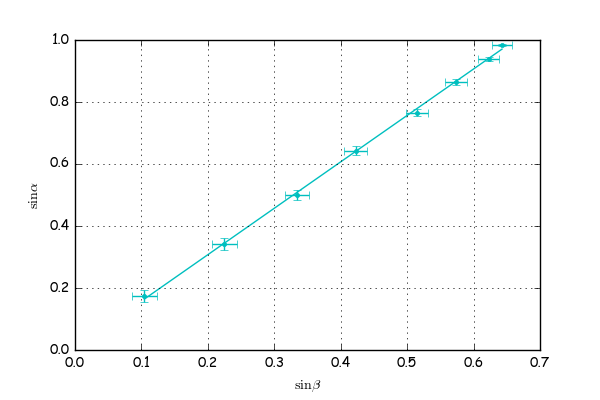
\includegraphics{./snella.png}
  \caption{}
  \label{}
\end{figure}

\subsection{Kąt graniczny}
Wyznaczony kąt graniczny wynosi: $\alpha_g = 44.0(1.1)^\circ$
\subsection{Prawo Malusa}
\begin{tabular}{lrrrrr}
\toprule
{} &$\theta[^\circ]$&u($\theta[^\circ]$)&I&$|z|$&u(I) \\
\midrule
0 &  0.0 & 1.118 & 0.900[mA] & 1[mA] & 0.025[mA] \\
1 & 15.0 & 1.118 & 0.820[mA] & 1[mA] & 0.025[mA] \\
2 & 30.0 & 1.118 & 0.620[mA] & 1[mA] & 0.025[mA] \\
3 & 45.0 & 1.118 & 0.400[mA] & 1[mA] & 0.025[mA] \\
4 & 60.0 & 1.118 & 0.1800[mA] & 0.3[mA] & 0.0075[mA] \\
5 & 75.0 & 1.118 & 43.0[$\mu$A] & 100[$\mu$A] & 2.5[$\mu$A] \\
6 &  90.0 &  1.118034 & 1.4[$\mu$A] &  3[$\mu$A] &  0.075[$\mu$A] \\
\bottomrule
\end{tabular}

\subsection{Współczynnik załamania}
\begin{tabular}{|l|c|c|}
  \toprule
  \hline
  metoda & współczynnik &niepewność \\
  pomiarowa & załamania & & \\\hline
  Prawo Snella & 1.498 & 0.022 \\\hline
  Kąt Brewstera&  &  \\\hline
  Kąt graniczny&  &  \\\hline
\bottomrule
\end{tabular}

\section{Analiza niepewności}

\section{Wnioski}
\paragraph{}...


\end{document}
